% !TeX TS-program = pdflatex


\documentclass[a4paper]{article}

% \usepackage[default]{fontsetup}

\usepackage{fancyhdr}
\usepackage{extramarks}
\usepackage{amsmath}
\usepackage{amsthm}
\usepackage{amsfonts}
\usepackage{tikz}
\usepackage[plain]{algorithm}
\usepackage{algpseudocode}
\usepackage{enumerate}
\usepackage{tikz}

\usetikzlibrary{automata,positioning}

%
% Basic Document Settings
%  

\topmargin=-0.2in
\evensidemargin=0in
\oddsidemargin=0in
\textwidth=6.5in
\textheight=9.5in
\headsep=0.25in

\linespread{1.1}

\pagestyle{fancy}
\lhead{\hmwkAuthorName}
\chead{\hmwkClass : \hmwkTitle}
\rhead{\firstxmark}
\lfoot{\lastxmark}
\cfoot{\thepage}

\renewcommand\headrulewidth{0.4pt}
\renewcommand\footrulewidth{0.4pt}

\setlength\parindent{0pt}

%
% Create Problem Sections
%

\newcommand{\enterProblemHeader}[1]{
    \nobreak\extramarks{}{Problem \arabic{#1} continued on next page\ldots}\nobreak{}
    \nobreak\extramarks{Problem \arabic{#1} (continued)}{Problem \arabic{#1} continued on next page\ldots}\nobreak{}
}

\newcommand{\exitProblemHeader}[1]{
    \nobreak\extramarks{Problem \arabic{#1} (continued)}{Problem \arabic{#1} continued on next page\ldots}\nobreak{}
    \stepcounter{#1}
    \nobreak\extramarks{Problem \arabic{#1}}{}\nobreak{}
}

\newcommand*\circled[1]{\tikz[baseline=(char.base)]{
		\node[shape=circle,draw,inner sep=2pt] (char) {#1};}}


\setcounter{secnumdepth}{0}
\newcounter{partCounter}
\newcounter{homeworkProblemCounter}
\setcounter{homeworkProblemCounter}{1}
\nobreak\extramarks{Problem \arabic{homeworkProblemCounter}}{}\nobreak{}

%
% Homework Problem Environment
%
% This environment takes an optional argument. When given, it will adjust the
% problem counter. This is useful for when the problems given for your
% assignment aren't sequential. See the last 3 problems of this template for an
% example.
%

\newenvironment{homeworkProblem}[1][-1]{
    \ifnum#1>0
        \setcounter{homeworkProblemCounter}{#1}
    \fi
    \section{Problem \arabic{homeworkProblemCounter}}
    \setcounter{partCounter}{1}
    \enterProblemHeader{homeworkProblemCounter}
}{
    \exitProblemHeader{homeworkProblemCounter}
}

%
% Homework Details
%   - Title
%   - Class
%   - Due date
%   - Name
%   - Student ID

\newcommand{\hmwkTitle}{Homework\ \#10}
\newcommand{\hmwkClass}{Probability \& Statistics for EECS}
\newcommand{\hmwkDueDate}{2024-12-17}
\newcommand{\hmwkAuthorName}{Wenye Xiong}
\newcommand{\hmwkAuthorID}{2023533141}


%
% Title Page
%

\title{
    \vspace{2in}
    \textmd{\textbf{\hmwkClass:\\  \hmwkTitle}}\\
    \normalsize\vspace{0.1in}\small{Due\ on\ \hmwkDueDate\ at 11:59}\\
	\vspace{4in}
}

\author{
	Name: \textbf{\hmwkAuthorName} \\
	Student ID: \hmwkAuthorID}
\date{}

\renewcommand{\part}[1]{\textbf{\large Part \Alph{partCounter}}\stepcounter{partCounter}\\}

%
% Various Helper Commands
%

% Useful for algorithms
\newcommand{\alg}[1]{\textsc{\bfseries \footnotesize #1}}
% For derivatives
\newcommand{\deriv}[1]{\frac{\mathrm{d}}{\mathrm{d}x} (#1)}
% For partial derivatives
\newcommand{\pderiv}[2]{\frac{\partial}{\partial #1} (#2)}
% Integral dx
\newcommand{\dx}{\mathrm{d}x}
% Alias for the Solution section header
\newcommand{\solution}{\textbf{\large Solution}}
% Probability commands: Expectation, Variance, Covariance, Bias
\newcommand{\E}{\mathrm{E}}
\newcommand{\Var}{\mathrm{Var}}
\newcommand{\Cov}{\mathrm{Cov}}
\newcommand{\Bias}{\mathrm{Bias}}

\begin{document}


% \maketitle
% \thispagestyle{empty}
% \pagebreak

\date{
Due on Dec. 17, 2024, 11:59 UTC+8}
\title{SI 140A-02  Probability \& Statistics for EECS, Fall 2024 \\
Homework 10}
\maketitle
Read all the instructions below carefully before you start working on the assignment, and before you make a submission.
\begin{itemize}
    \item You are required to write down all the major steps towards making your conclusions; otherwise you may obtain limited points of the problem.
    \item Write your homework in English; otherwise you will get no points of this homework.
    \item Any form of plagiarism will lead to $0$ point of this homework. 
\end{itemize}
\newpage
\begin{homeworkProblem}[1]
Let $U_{i} \sim \operatorname{Unif}(0,1), i \geq 1$ be i.i.d. random variables. Define $N$ as follows:
$$
N=\max \left\{n: \prod_{i=1}^{n} U_{i} \geq e^{-1}\right\}
$$
\begin{enumerate}[(a)]
\item Estimate $\mathrm{E}(N)$ by generating 5000 samples of $N$ and then use the sample mean.
\item Estimate $\operatorname{Var}(N)$.
\item Estimate $P(N=i)$, for $i=0,1,2,3$.
\item Can you find the exact distribution of $N$ ?
\end{enumerate}
\end{homeworkProblem}

\newpage

\begin{homeworkProblem}[2]
    Visualization of Bivariate Normal Distribution with correlation coefficient $\rho$
    \begin{enumerate}[(a)]
        \item Use the following transformation to generate samples from bivariate Normal distribution with correlation coefficient $\rho$ :
        $$
        \begin{aligned}
        & X=Z \\
        & Y=\rho Z+\sqrt{1-\rho^{2}} W
        \end{aligned}
        $$
        where $-1<\rho<1, Z$ and $W$ are i.i.d. random variables satisfying $\mathcal{N}(0,1)$.
        \item Plot the joint pdf function and the corresponding contour(or isocontour) as the following figure:\\
        \begin{figure*}[htb]
            \centering
            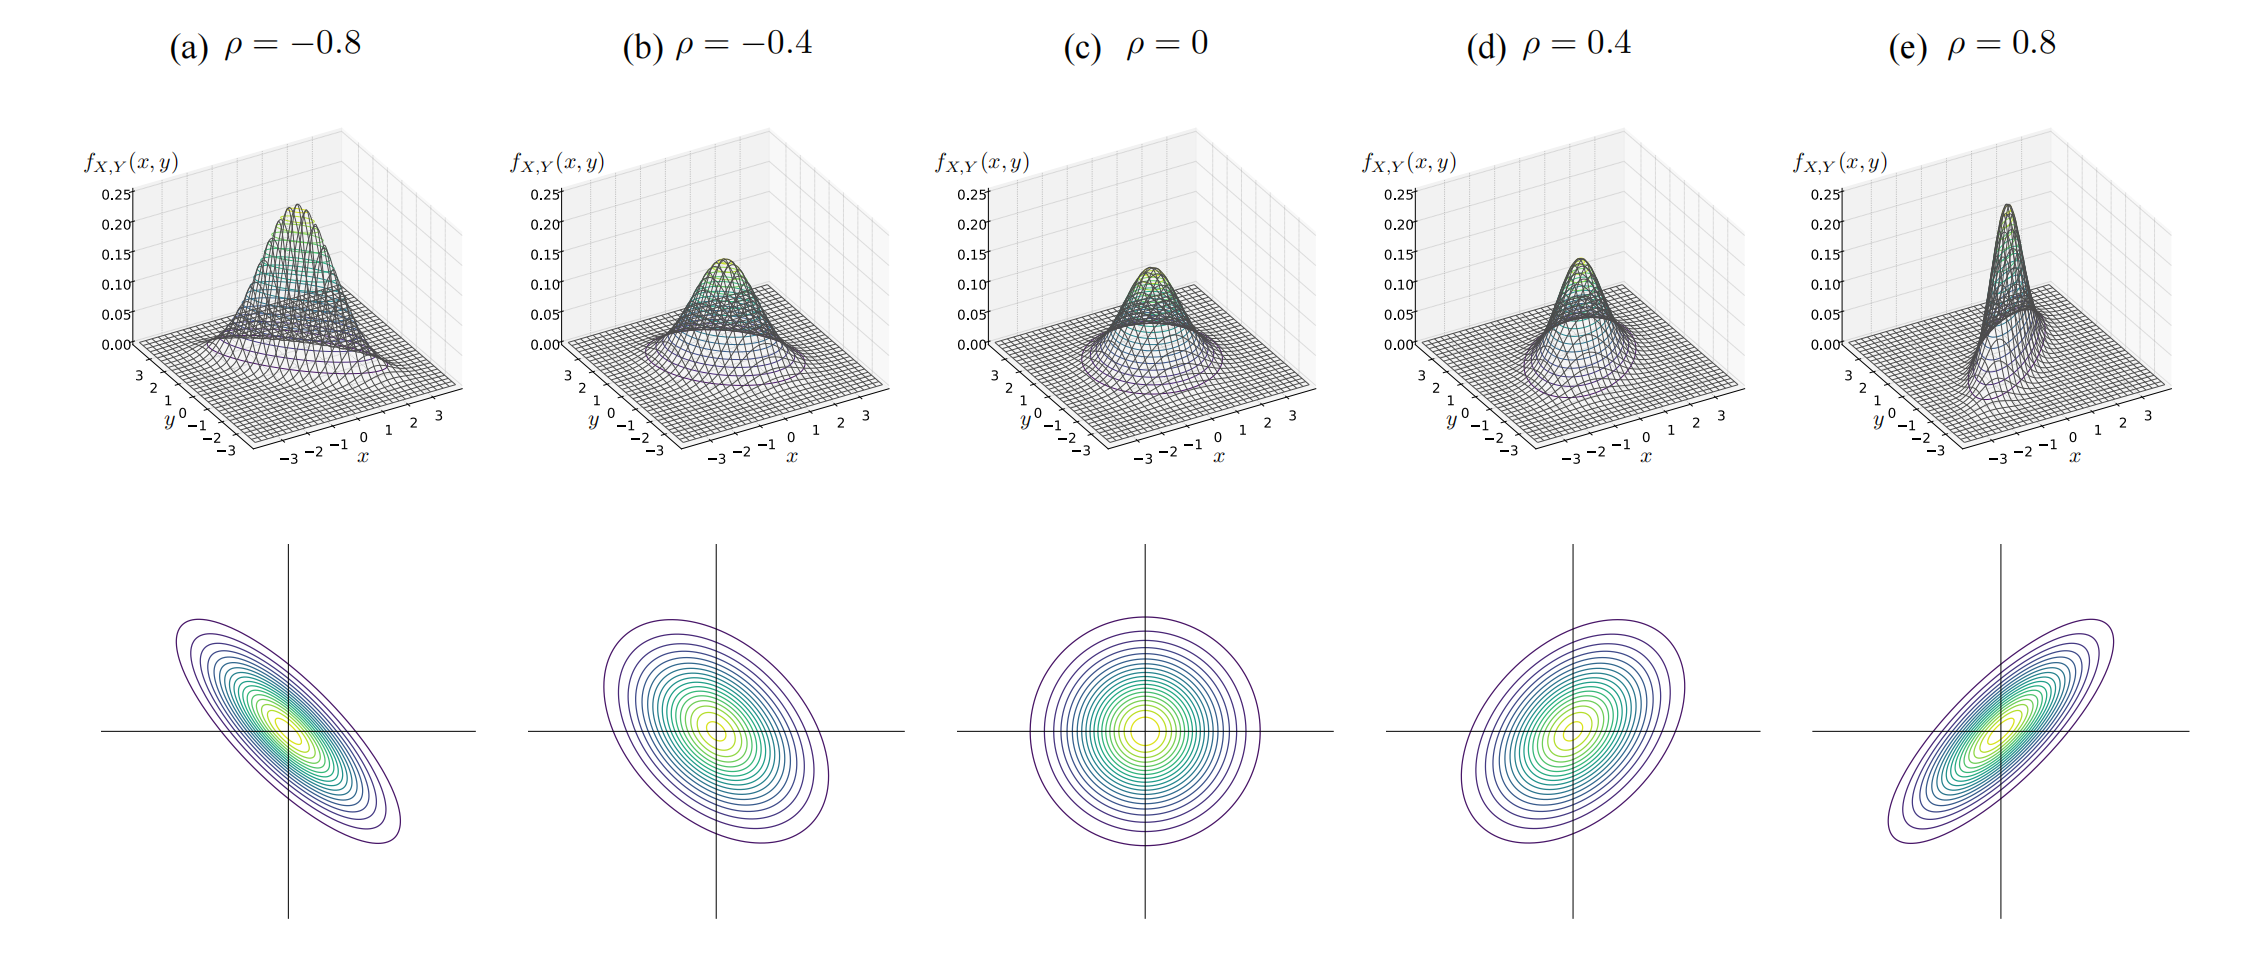
\includegraphics[width=1\linewidth]{图片1.png}
            
        \end{figure*}
    \end{enumerate}
\end{homeworkProblem}

\newpage

\begin{homeworkProblem}[3]
     Let $X_{1} \sim \operatorname{Expo}\left(\lambda_{1}\right), X_{2} \sim \operatorname{Expo}\left(\lambda_{2}\right)$ and $X_{3} \sim \operatorname{Expo}\left(\lambda_{3}\right)$ be independent.
     \begin{enumerate}[(a)]
         \item Find $E\left(X_{1} \mid X_{1}>2024\right)$
         \item Find $E\left(X_{1} \mid X_{1}<1997\right)$
         \item Find $E\left(X_{1}+X_{2}+X_{3} \mid X_{1}>1997, X_{2}>2014, X_{3}>2025\right)$ in terms of $\lambda_{1}, \lambda_{2}, \lambda_{3}$.
     \end{enumerate}
         
\end{homeworkProblem}

\newpage

\begin{homeworkProblem}[4]
    Let $X$ and $Y$ be two continuous random variables with joint PDF
$$
f_{X, Y}(x, y)= \begin{cases}6 x y & \text { if } 0 \leq x \leq 1,0 \leq y \leq \sqrt{x} \\ 0 & \text { otherwise }\end{cases}
$$

    \begin{enumerate}[(a)]
        \item Find the marginal distributions of $X$ and $Y$. Are $X$ and $Y$ independent?
        \item Find $E[X \mid Y=y]$ and $\operatorname{Var}[X \mid Y=y]$ for $0 \leq y \leq 1$.
        \item Find $E[X \mid Y]$ and $\operatorname{Var}[X \mid Y]$.
    \end{enumerate}
\end{homeworkProblem}

\newpage

\begin{homeworkProblem}[5]
    Let $X$ be a discrete r.v. whose distinct possible values are $x_{0}, x_{1}, \ldots$, and let $p_{k}=$ $P\left(X=x_{k}\right)$. The entropy of $X$ is $H(X)=\sum_{k=0}^{\infty} p_{k} \log _{2}\left(1 / p_{k}\right)$.
    \begin{enumerate}[(a)]
        \item Find $H(X)$ for $X \sim \operatorname{Geom}(p)$.
        \item Let $X$ and $Y$ be i.i.d. discrete r.v.s. Show that $P(X=Y) \geq 2^{-H(X)}$.
    \end{enumerate}
\end{homeworkProblem}

\newpage
\begin{homeworkProblem}[6]
    Instead of predicting a single value for the parameter, we give an interval that is likely to contain the parameter: A $1-\delta$ confidence interval for a parameter $p$ is an interval $[\hat{p}-\epsilon, \hat{p}+\epsilon]$ such that ${Pr}(p \in[\hat{p}-\epsilon, \hat{p}+\epsilon]) \geq 1-\delta$. Now we toss a coin with probability $p$ landing heads and probability $1-p$ landing tails. The parameter $p$ is unknown and we need to estimate its value from experiment results. We toss such coin $N$ times. Let $X_{i}=1$ if the $i$ th result is head, otherwise 0 . We estimate $p$ by using

$$
\hat{p}=\frac{X_{1}+\ldots+X_{N}}{N}
$$

Find the $1-\delta$ confidence interval for $p$, then discuss the impacts of $\delta$ and $N$.
\begin{enumerate}[(a)]
    \item  Method 1: Adopt Chebyshev inequality to find the $1-\delta$ confidence interval for $p$, then discuss the impacts of $\delta$ and $N$.
    \item Method 2: Adopt Hoeffding bound to find the $1-\delta$ confidence interval for $p$, then discuss the impacts of $\delta$ and $N$.
    \item Discuss the pros and cons of the above two methods.
\end{enumerate}
\end{homeworkProblem}

\newpage
\begin{homeworkProblem}[7](\textbf{Optional Challenging Problem})
    We consider the progressive Monty Hall problem. This time we assume there are $n$ identical doors, where $n$ is an integer satisfying $n \geq 3$. One door conceals a car, the other $n-1$ doors conceal goats. You choose one of the doors at random but do not open it. Monty then opens a door he knows to conceal a goat, always choosing randomly among the available doors. At this point he gives you the option either of sticking with your original door or switching to one of the remaining doors. You make your decision. Monty now eliminates another goat-concealing door (at random) and once more gives you the choice either of sticking or switching. This process continues until only two doors remain in play. What strategy should you follow to maximize your chances of winning? We consider three strategies: (1) Select a door at random and stick with it throughout. (2) Select a door at random, then switch doors at every opportunity, choosing your door randomly at each step. (3) Select a door at random, stick with your first choice until only two doors remain, and then switch. When $n=10$ and $n=1000$, \textbf{please run simulations to estimate the winning probability of each strategy. Check which strategy is best and provide the corresponding intuition.}
\end{homeworkProblem}


\end{document}